\subsection{Aantal trainingssessies}
Intu\"itie zegt dat hoe meer gelegenheden het netwerk krijgt om te trainen, hoe beter het netwerk wordt. Hier willen we kijken wat de bovengrens is en tot waar extra trainingssessies weinig invloed hebben op het netwerk.

\begin{table}[ht]
    \centering
      $\begin{array}{c||c|c |}
        \text{Aantal trainingssessies} & \text{Aantal correct} & \text{Percentage \% correct} \\ \hline
        1 & 0 & 0 \\ \hline
        100001 & 15 & 30 \\ \hline
        200001 & 36 & 72 \\ \hline
        300001 & 38 & 76 \\ \hline
        400001 & 44 & 88 \\ \hline
        500001 & 41 & 82 \\ \hline
        600001 & 42 & 84 \\ \hline
        700001 & 43 & 86 \\ \hline
        800001 & 46 & 92 \\ \hline
        900001 & 45 & 90 \\ \hline
        1000001 & 43 & 86 \\ \hline
        1100001 & 48 & 96 \\ \hline
        1200001 & 46 & 92 \\ \hline
        1300001 & 48 & 96 \\ \hline
        1400001 & 46 & 92 \\ \hline
        1500001 & 46 & 92 \\ \hline
      \end{array}$
    \caption{Aantal correcte antwoorden over 50 executies met verschillende aantallen trainingssessies}
    \label{tab:training}
\end{table}

\begin{figure}[ht!]
    \centering
    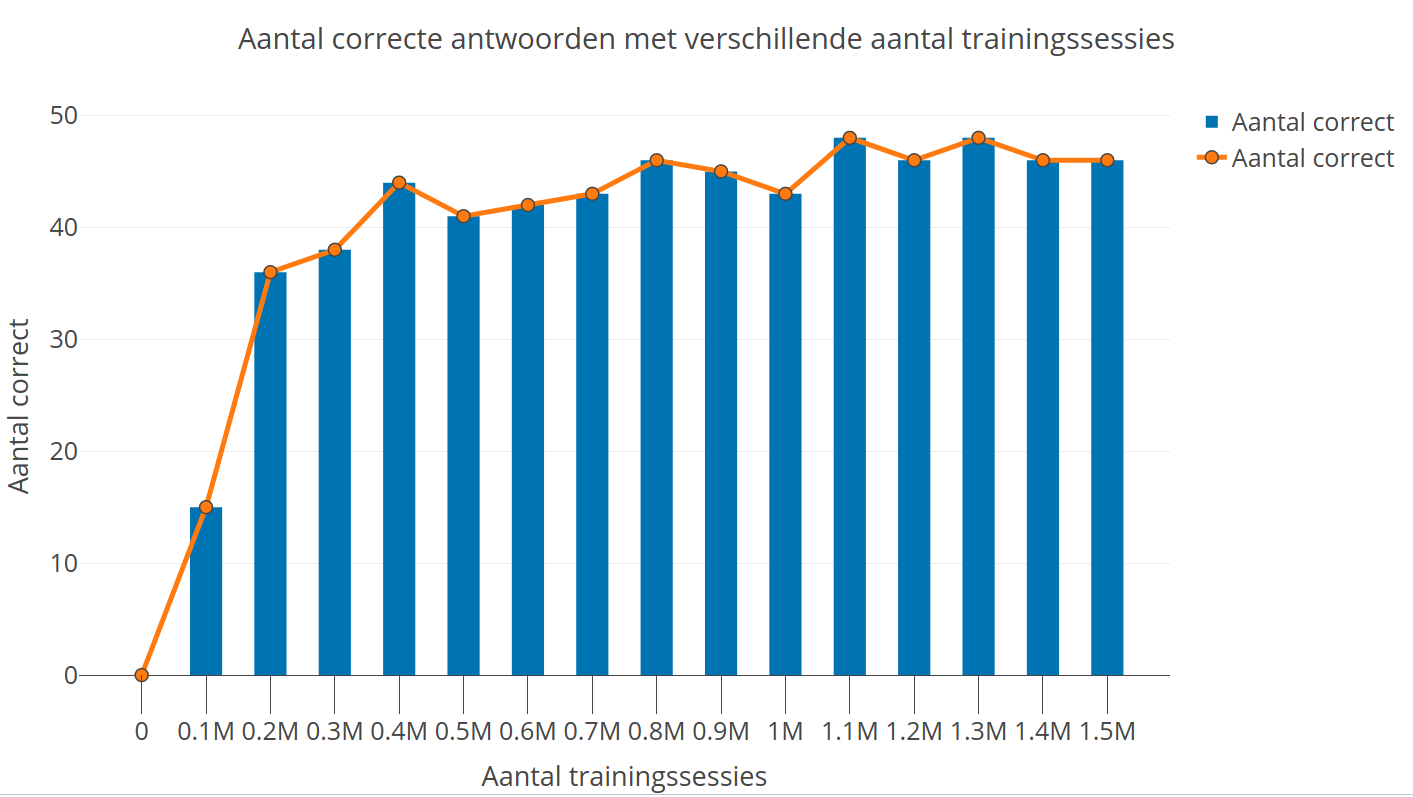
\includegraphics[scale=0.3]{graphs/training.png}
    \caption{Grafiek van Tabel \ref{tab:training}}
    \label{fig:training}
\end{figure}
